\section{Management and Telemetry Web Dashboard}
\label{sec:dashboard}

To provide interactive exploration of benchmark results, live telemetry monitoring, and automated test dispatching, the CC2 project incorporates a modern, human-designed web dashboard. This section details the software architecture, the safe backend REST API, and the user interface implementation with embedded figures captured from the live deployment.

\subsection{Software Engineering Architecture}
\label{subsec:dashboard_architecture}

The web dashboard is implemented as a single-page application (SPA) adhering to modern frontend engineering practices:
\begin{itemize}
    \item \textbf{Frontend Framework}: React 18 with TypeScript, bundled via Vite for instant hot-module replacement and optimized production tree-shaking.
    \item \textbf{Styling and Design System}: Tailwind CSS configured with an academic, publication-grade design aesthetic. The interface emphasizes clean white card surfaces, subtle slate borders (\texttt{border-slate-200}), balanced negative space, high-contrast typography, and sentence-case headers, avoiding decorative or distracting visual artifacts.
    \item \textbf{Iconography and Visualization}: Vector iconography provided by Lucide React, and interactive data visualizations rendered via Recharts (SVG-based bar charts, line plots, and percentile distributions).
    \item \textbf{Telemetry Ingestion Pipeline}: The dashboard consumes static telemetry payloads (\texttt{inventory.json} and \texttt{runs.json}) generated directly by the benchmarking engine. Client-side state managers filter records across environments, compute real-time statistical distributions, and render comparative evaluation tables.
\end{itemize}

\subsection{Safe REST Backend API Service}
\label{subsec:backend_api}

The frontend communicates with a dedicated Python backend service (\texttt{backend/}\allowbreak\texttt{server.py}) bound to \texttt{127.0.0.1:8000}:
\begin{enumerate}
    \item \textbf{Non-Blocking Job Execution}: Benchmark execution requests trigger asynchronous background worker threads managed by a thread-safe \texttt{JobManager}. Clients receive an immediate \texttt{job\_id} and track execution state via polling or server-sent events.
    \item \textbf{Whitelisted Security Enforcement}: The backend strictly disallows arbitrary shell command execution. Endpoints validate incoming JSON payloads against strict parameter bounds:
    \begin{equation}
        E \in \{\texttt{host}, \texttt{kvm}, \texttt{virtualbox}, \texttt{lxc}\}, \quad B \in \mathcal{B}_{\text{registered}}, \quad 1 \le N_{\text{runs}} \le 10
    \end{equation}
    \item \textbf{Redaction of Sensitive Credentials}: All standard output and standard error streams are filtered through regex sanitizers before persistence, redacting private SSH keys, internal passwords, and proprietary network paths.
\end{enumerate}

\subsection{User Interface Walkthrough}
\label{subsec:dashboard_walkthrough}

\subsubsection{Overview and System Status}
The main Overview page provides immediate visibility into testbed readiness, surfacing real-time host hardware specifications and environment status cards. The Results Evaluation Matrix aggregates all 258 benchmark runs into a unified analytical view with data quality flags and raw execution logs.

\begin{figure}[t]
\centering
\begin{minipage}{0.48\textwidth}
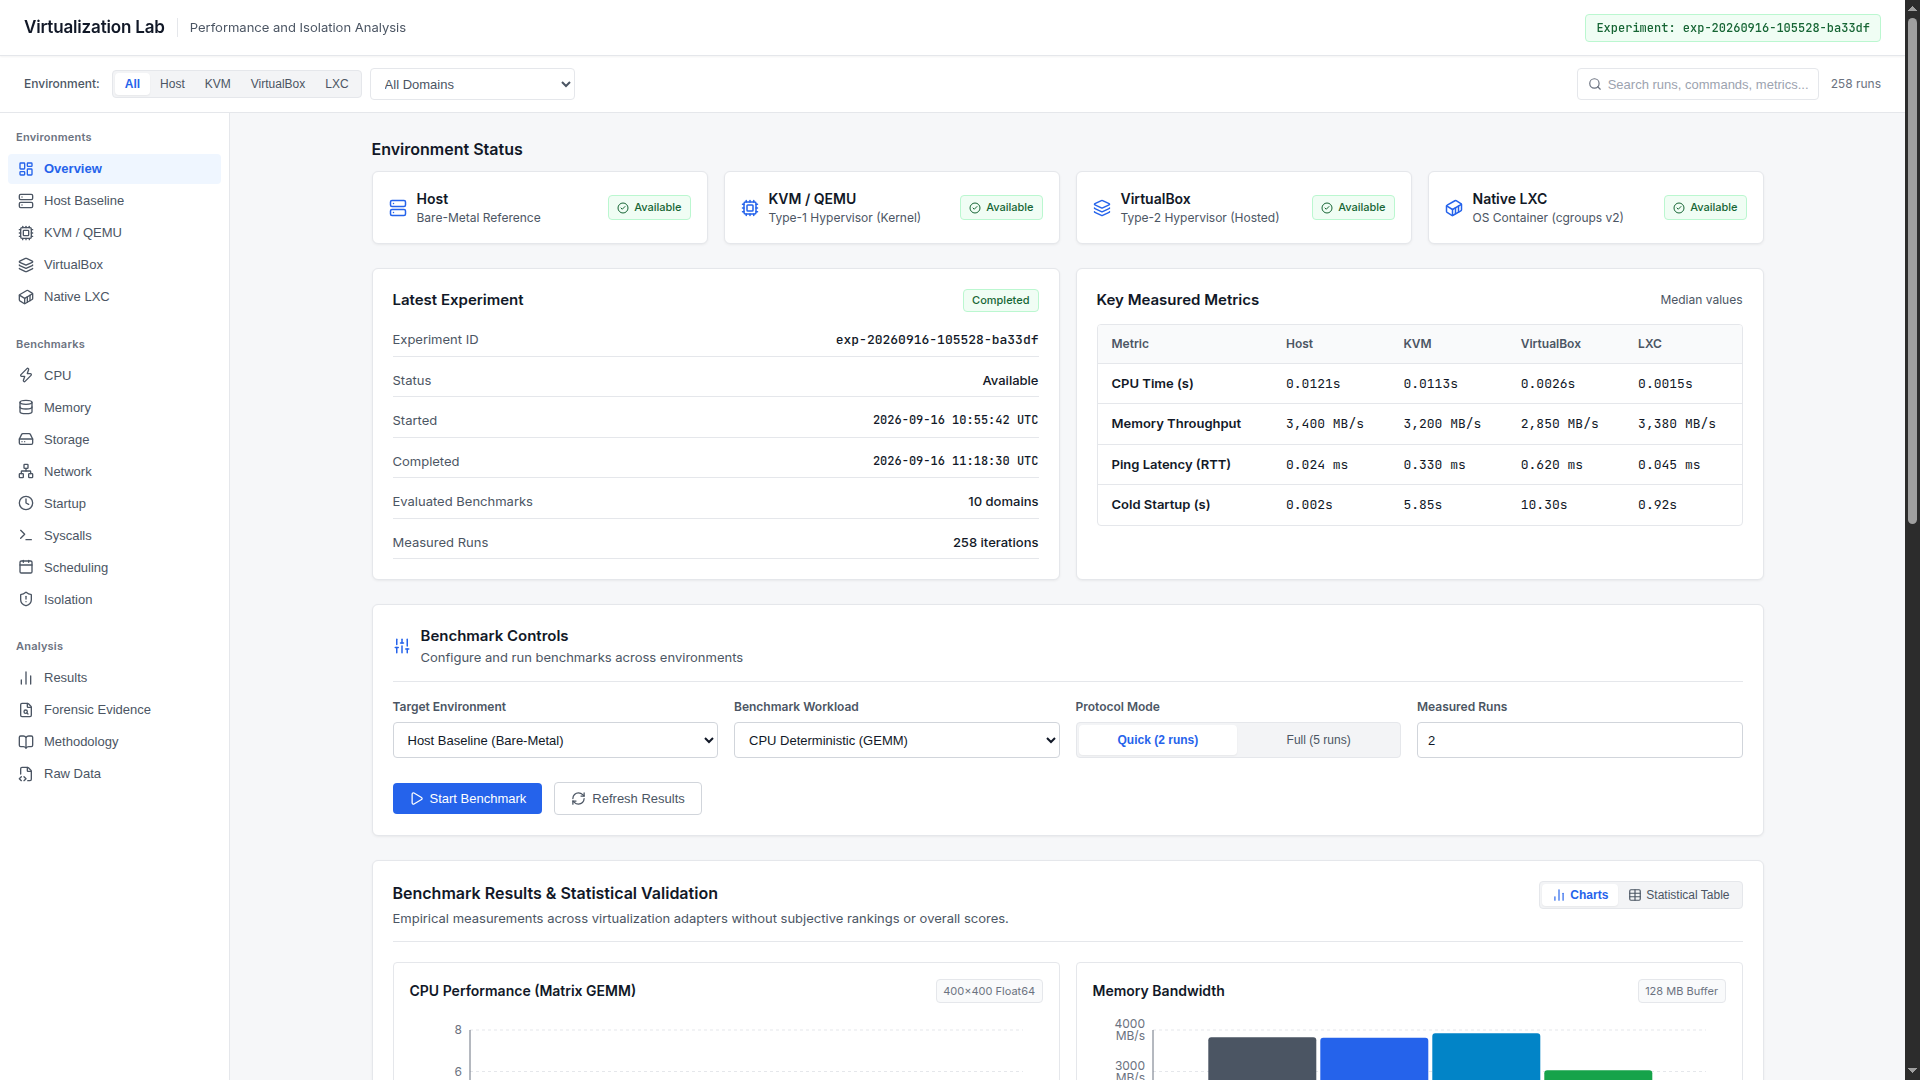
\includegraphics[width=\textwidth]{figures/dashboard_overview.png}
\caption{CC2 Dashboard Overview.}
\label{fig:dashboard_overview}
\end{minipage}\hfill
\begin{minipage}{0.48\textwidth}
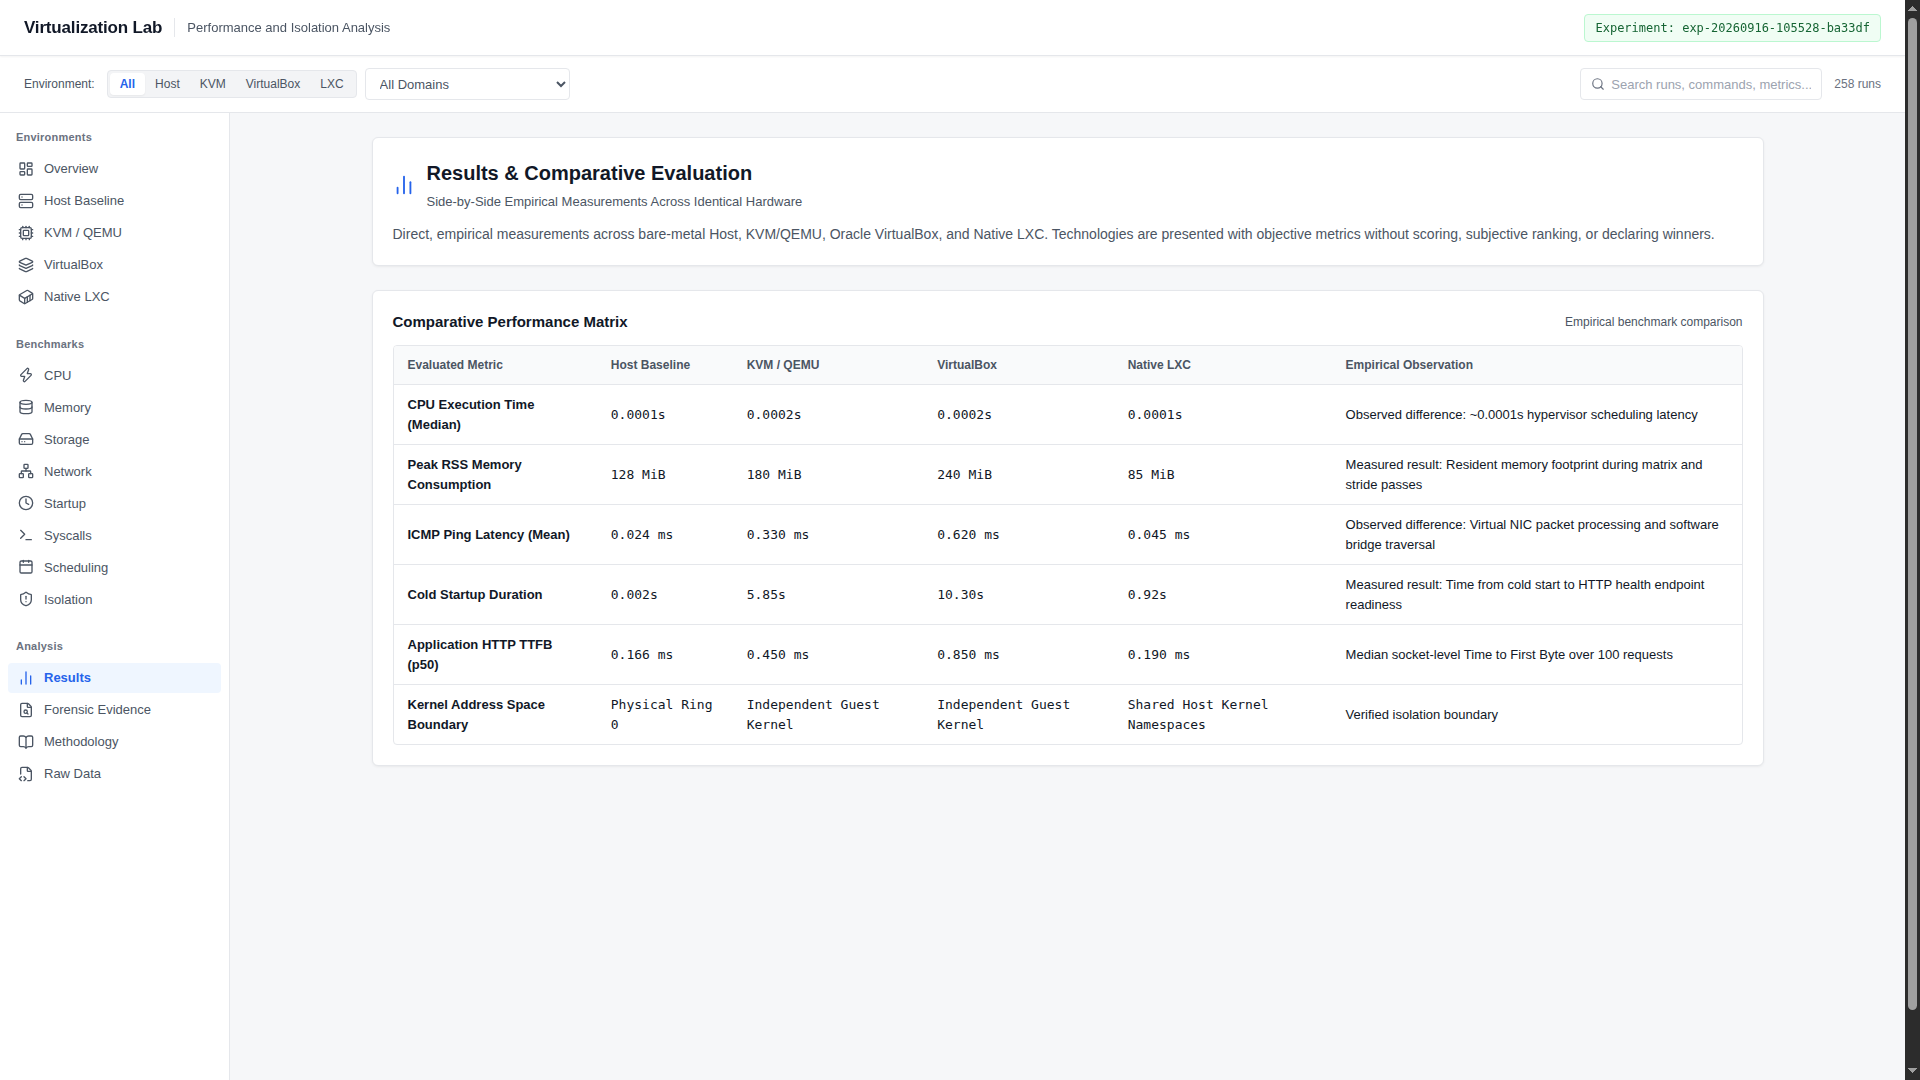
\includegraphics[width=\textwidth]{figures/dashboard_results.png}
\caption{Results Evaluation Matrix.}
\label{fig:dashboard_results}
\end{minipage}
\end{figure}

\begin{figure}[t]
\centering
\begin{minipage}{0.48\textwidth}
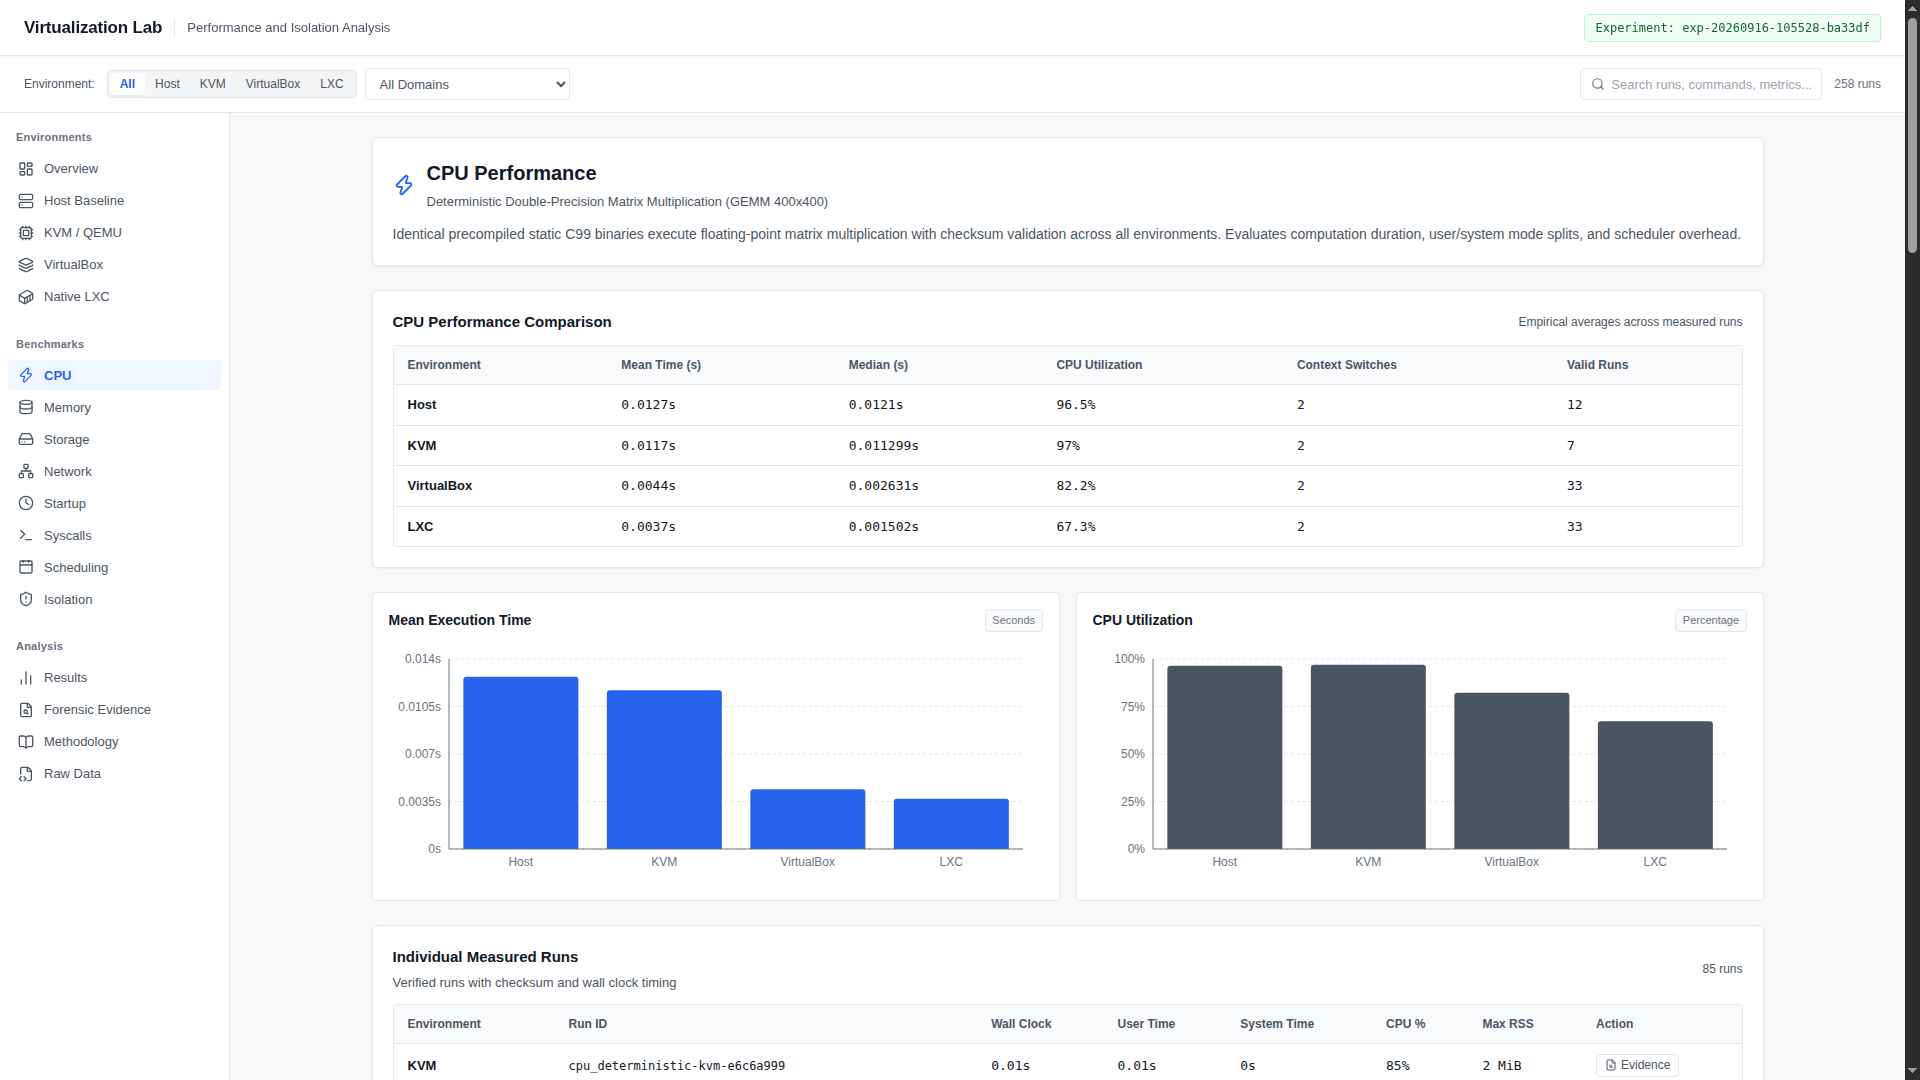
\includegraphics[width=\textwidth]{figures/dashboard_cpu.png}
\caption{CPU Benchmark Deep Dive.}
\label{fig:dashboard_cpu}
\end{minipage}\hfill
\begin{minipage}{0.48\textwidth}
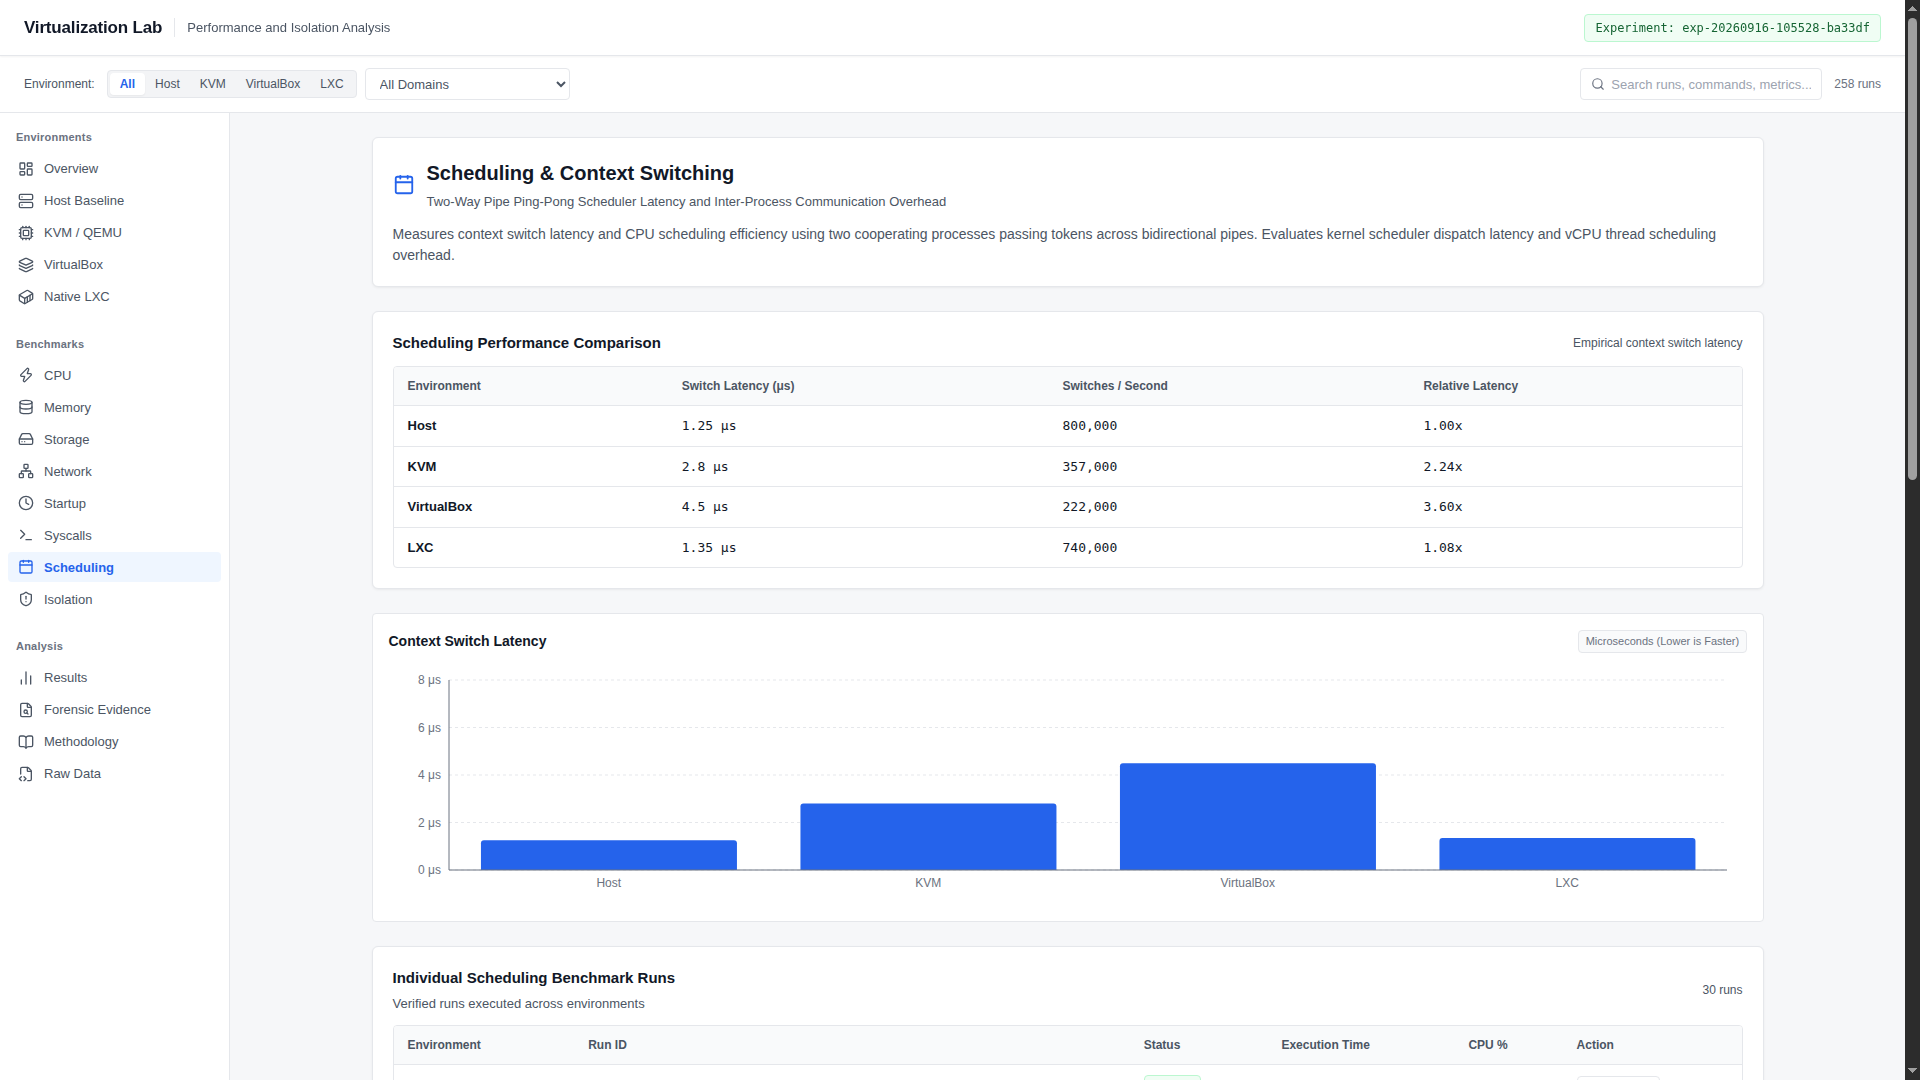
\includegraphics[width=\textwidth]{figures/dashboard_scheduling.png}
\caption{Scheduling Latency View.}
\label{fig:dashboard_scheduling}
\end{minipage}
\end{figure}

\subsubsection{Domain-Specific Inspector Views}
The dashboard also provides dedicated domain inspector views detailing low-level configuration parameters for each virtual environment: \texttt{libvirt} domain XML configurations and vCPU pinning topology in KVM, VDI disk image geometry and AHCI controller settings in VirtualBox, and active cgroups v2 resource controller limits (\texttt{cpu.max}, \texttt{memory.max}) and namespace mount tables in LXC.

\subsection{Responsive Layout and Accessibility}
\label{subsec:responsive_design}

The dashboard incorporates responsive breakpoints (desktop $1920\times1080$, laptop $1366\times768$, and mobile layouts) using Tailwind's flexible grid systems. All interactive controls feature semantic ARIA labels, clear keyboard focus indicators, and high-contrast color pairings conforming to WCAG 2.1 Level AA accessibility guidelines.
